\section{Proxy Architecture}
\label{sec:netshaper-proxy-arch}

\begin{figure}[!htb]
    \centering
    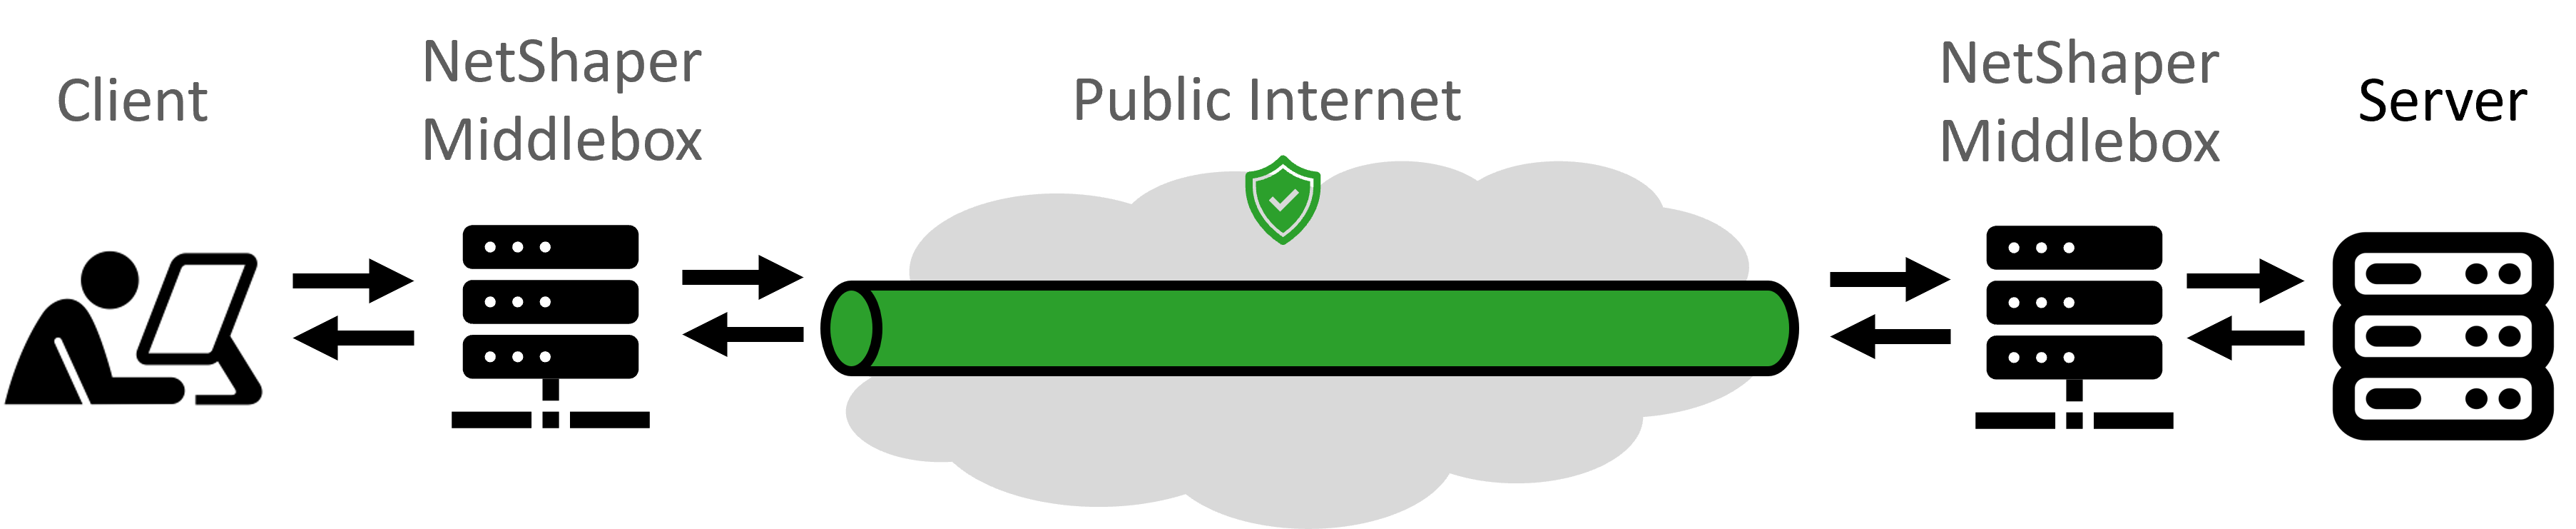
\includegraphics[width=\columnwidth]{figures/netshaper/netshaper-setup.png}
    \caption{NetShaper's Tunnel Setup}
    \label{fig:netshaper-setup}
\end{figure}

We designed NetShaper as a modular system that can be deployed using a pair of middleboxes, forming a forward and reverse proxy pair (see \Cref{fig:netshaper-setup}). 
Here, we describe in detail the architecture of the proxy setup and defer the discussion regarding the design of the middlebox to \Cref{sec:netshaper-middlebox-design}. 

When using NetShaper, all clients communicate with the servers using three piecewise connections: 
(\textit{i}) between the client and the client-side middlebox, 
(\textit{ii}) between the client-side middlebox and the server-side middlebox, and
(\textit{iii}) between the server-side middlebox and the server.

For connection \textit{i} and \textit{iii}, NetShaper relies on standard TCP/UDP protocols. However, for connection \textit{ii} (i.e. to proxy the payload), NetShaper utilises QUIC. 
Using QUIC to proxy the payload avoids the TCP meltdown problem [??] that occurs when tunnelling TCP via TCP.
In addition, using QUIC also avoids the problem of an observer/attacker being able to distinguish between payload and padding that would occur when TCP was tunnelled via UDP (as the end host would retransmit payload, but the padding would not be retransmitted).

\paragraph{Setup.}
In order to be able to proxy end host traffic via NetShaper, the middleboxes need to be configured. 
The middleboxes first establish an encrypted QUIC connection between them, with user-specified reliability semantics.
Once the QUIC connection is established, NetShaper initialises three types of QUIC streams: Control, Data (Payload), and Dummy (Padding).
One \textit{control} stream is used to transmit messages regarding connection establishment or termination by the end host.
One \textit{dummy} stream is used for adding padding to the payload whenever necessary, based on the output of $f_{DP}$
\footnote{We avoid the use of PADDING frames in QUIC as they do not elicit acknowledgements and hence are distinguishable from the payload \cite{quic_rfc}.}.

\paragraph{Supporting multiple end hosts.}
As we discussed in \Cref{subsec:netshaper-background-quic}, QUIC supports multiple streams in the same connection.
Using this, NetShaper can proxy the payload of multiple end hosts through a single QUIC connection between a pair of middleboxes.

While QUIC can support arbitrary initialisation and termination of streams, each stream has an associated header, which would increase the total transmission size.
For example, when transmitting two bytes in a single stream, the total transmission size would be $2 + S_{header}$.
However, when transmitting two streams of one byte each, the total transmission size would be $2 + 2*S_{header}$. 
An adversary may be able to distinguish between these two scenarios.
In order to avoid such a situation, NetShaper fixes and initialises a fixed number of streams per QUIC connection during the setup phase.
NetShaper assigns an unused stream to the client whenever a new client connects to the middlebox.
Similarly, NetShaper marks a stream as unused when an end host terminates the connection.

\endinput